% !TEX root = ./HTNotes-Demo.tex
% !TEX program = xelatex
\begin{flushright}
文/似雪飞扬
\end{flushright}

\section{预备知识}
  \subsection*{初等函数与分段函数}
    \begin{defn}
      由基本初等函数经过有限次四则运算和复合运算得到的,可以只用一个式子表达的函数称为初等函数.
    \end{defn}
    \begin{defn}
      由多个定义在不同区间上的式子组合在一次表达的函数称为分段函数.
    \end{defn}
    几点说明:
    \begin{enumerate}[label=(\arabic*)]
      \item 分段函数不一定不是初等函数.

      举例:$f(x) = \abs{x} =
      \begin{cases}
        x, & x \ge 0 \\
        -x, & x < 0
      \end{cases}
      = \sqrt{x^2}, x \in \mathbb{R}$.

      一般地,若分段函数$f(x)$的各段定义区间是连着的,且 是连续函数,则$f(x)$是初等函数.
      \item 基本初等函数在定义域上处处连续.
      \item 初等函数在各段定义区间上分别处处连续(在分段点处可能间断也可能连续).

      举例:$f(x) =\sin \dfrac{1}{x}, x \in \mathbb{R}$在$(0,+\infty)$, $(-\infty,0)$上均连续,而在原点处振荡间断.

      这个命题不放在微分学部分是因为一般将其作为不证自明的基本命题.
    \end{enumerate}

\section{一元函数微分学部分}
~ \subsection{连续、间断与可导}
    \hspace*{2em}讨论点态连续的前提是函数在该点邻域内有定义,讨论点态间断的前提是函数在该点去心邻域内有定义. 例如,对$f\left( x \right) =x$, $x\in \mathbb{Q}$讨论连续性是无意义的.

    \hspace*{2em}间断点的分类标准是两侧极限是否存在. 若函数在某点处间断但两侧极限均存在,则将该点定义为第一类间断点,并按两侧极限是否相等分为可去间断点和跳跃间断点(立即可知对于可去间断点必定有函数在该点处无定义的结论);若函数在某点两侧的极限至少有一侧不存在(或者两侧都不存在. 显然第二类间断点对该点是否有定义并无要求,可以有也可以没有),则将该点定义为第二类间断点,并按单侧极限不存在的方式是趋于无穷还是振荡将该侧间断分为无穷间断和振荡间断.

    \hspace*{2em}举例:
    $$f\left( x \right) =
    \begin{cases}
      \sin \dfrac{1}{x}, & x \ne 0\\
      0, & x=0 \\
    \end{cases}$$
    在原点处振荡间断,图像如\autoref{fig:一个常见振荡间断点的例子.}所示. 这也是也是振荡间断点最常用的例子.
    \begin{figure}[!h]
      \centering
      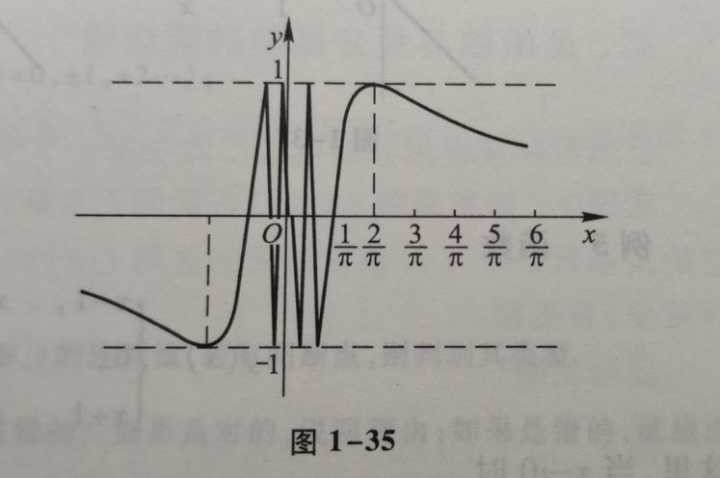
\includegraphics[width=.3\textwidth]{App2_1}
      \caption{一个常见振荡间断点的例子.}\label{fig:一个常见振荡间断点的例子.}
    \end{figure}

    几点说明:
    \begin{enumerate}[label={(\arabic*)}]
      \item  非初等函数可能只在某些点处连续,也可能处处不连续,但不可能几乎处处
      \footnote{“几乎处处”是数学分析中的一个说法. 若某性质P对于集合 中的每一个元素都成立,称性质P在集合 上处处成立;若性质P对于集合 中的每一个元素都成立,其中 是零测集,则称性质P在集合 上几乎处处成立. 这个概念我们还将会在积分学部分再次遇到.}
       连续.

      举例:狄利克雷(Dirichlet)函数
      \[ D\left( x \right) =\begin{cases}
        \text{1,}&    x\in \mathbb{Q}\\
        0, &    x\in \mathbb{R}\backslash\mathbb{Q}\\
      \end{cases} \]
      处处不连续,略作变化即可得到只在原点处连续的函数
      $$f\left( x \right) =x\rd \left( x \right) =\begin{cases}
        x,&   x\in \mathbb{Q}\\
        0, &    x\in \mathbb{R}\backslash\mathbb{Q}\\
      \end{cases}$$

      事实上,初等函数才是在其定义域上几乎处处连续的
      \footnote{举例:$\tan x$和$\tan \frac{1}{x}$在$\mathbb{R}$上几乎处处连续.}
      .

      \item 处处连续的函数在某点处不一定可导,甚至可能处处不可导.

      举例:$f\left( x \right) =
      \begin{cases}
        x\sin \dfrac{1}{x}, & x \ne 0\\
        0, & x=0 \\
      \end{cases}$
      处处连续但在原点处不可导;
      魏尔斯特拉斯(Weierstrass)函数
      $$f\left( x \right) =\sum_{i=1}^{\infty}{a^n\cos \left( b^n\pi x \right)}\left( a\in \left( 0, 1 \right) ,b=2k+\text{1,}k\in \mathbb{N},ab>1+\frac{3}{2}\pi \right) $$
      \begin{figure}[!h]
        \centering
        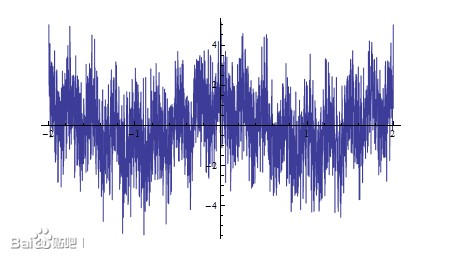
\includegraphics[width=.3\textwidth]{App2_2}
        \caption{Weierstrass函数图像示意图.}\label{fig:Weierstrass函数图像示意图.}
      \end{figure}
      处处连续但无处可导,如\ref{fig:Weierstrass函数图像示意图.}所示;

      \item 处处可导的函数,它的导函数在其定义域上不一定连续.

      举例:$f\left( x \right) =
      \begin{cases}
        x^2 \sin \dfrac{1}{x}, & x \ne 0\\
        0, & x=0 \\
      \end{cases}$.

      \item 函数在某点处的左右导数均存在(但不一定相等),则可以推出函数在该点连续.

      简单证明如下:由左右导数存在可知$\Delta y=\begin{cases}
        y'_-\left( x_0 \right) \cdot \Delta x,&   \Delta x<0\\
        y'_+\left( x_0 \right) \cdot \Delta x,&   \Delta x>0\\
      \end{cases}\rightarrow 0\left( \Delta x\rightarrow 0 \right)$.

      \item 函数在某点处可导,不一定在该点去心邻域内连续.

      举例:借助狄利克雷函数构造$f\left( x \right) =x^2\text{D}\left( x \right)$在$x=0$处可导,但在$\mathbb{R}\backslash\{0\}$内处处不连续.

      \item 导函数在某点处的极限存在,不能推知函数在该点连续.

      举例:$f\left( x \right) =\left[ \sgn \left( x \right) \right] ^2=\begin{cases}  \text{1,}&    x\ne 0\\  0, &    x=0\\\end{cases}$.

      \item 导函数在某点处的极限存在,且函数在该点处连续,则函数在该点可导,且导函数在该点连续.

      这个命题称为导数极限定理,可以通过洛必达法则证明:设$f(x)$在$x = x_0$处连续,且$\lim\limits_{x \to x_0} f'(x)$存在,则
      \[ f'\left( x_0 \right) =\underset{x\rightarrow x_0}{\lim}\frac{f\left( x \right) -f\left( x_0 \right)}{x-x_0}\xlongequal{\text{L'Hospital}}\underset{x\rightarrow x_0}{\lim}\frac{f'\left( x \right)}{1}=\underset{x\rightarrow x_0}{\lim}f'\left( x \right) \]

      \item 连续性是介值性
      \footnote{介值定理:定义在区间上的连续函数,其值域必定也是区间(可缩为一点). 该定理可借助零点存在定理,由构造函数法证明. 介值性:设$I_f=\left[ a,b \right], $若$\forall a\le x_1<x_2\le b,f\left( x_1 \right) \ne f\left( x_2 \right)$, $f\left( x \right) $可取到$f\left( x_1 \right) \text{和}f\left( x_2 \right) $之间的任意值,称$f$在$[a,b]$上具有介值性.}
      的充分不必要条件.

      举例:已在前文出现过的$f\left( x \right) =x\text{D}\left( x \right) =\begin{cases}
        x,&   x\in \mathbb{Q}\\
        0, &    x\in \mathbb{R}\backslash\mathbb{Q}\\
      \end{cases}$还告诉我们,区间上的函数即使处处不连续,也可以具有介值性.

      另外一个非常有意思的例子是导数介值定理(也被称为达布中值定理):闭区间上可导的函数,其导函数可以取到该区间两端点处导数值之间的一切值,即导函数具有介值性. 可以通过费马引理证明之,此处不再赘述.
    \end{enumerate}

  \subsection{可导、极值与单调性}
    \begin{enumerate}[label=(\arabic*)]

      \item 连续函数在某点处取得极值,不能推知函数在该点邻域内的单调性.
      举例:魏尔斯特拉斯函数在原点处取得极大值,但在原点的任意单侧去心邻域内不单调.

      \item 连续函数在某点可导且导数不为0,不能推知函数在该点邻域内的单调性.

      如2004年考研数学一8题/数学二10题:设函数$f(x)$连续,且$f'(0)>0$,则存在$\delta>0$,使得(\qquad)
      \options{在$(0,\delta)$内单调增加}
      {在$(-\delta,0)$内单调减少}
      {对任意的$x \in (0,\delta)$有$f(x)>f(0)$}
      {对任意的$x \in (-\delta,0)$有$f(x)>f(0)$}
      答案:C. 对错解AB构造反例:$f\left( x \right) =\begin{cases}
        x^2\sin \dfrac{1}{x} + \dfrac{x}{2}, & x\ne 0, \\
        0, & x=0 \\
      \end{cases}$.

      \item 可导函数在某点处导数为0是其在该点处取得极值的必要不充分条件.

      该命题可以通过费马引理证明,此处不加赘述.

      \item 函数在某点处连续、在该点去心邻域内可导且导函数在该点两侧变号,是其在该点处取得极值的第一充分不必要条件.

      这一点也警示我们,讨论极值点时不能仅看函数的导数为0的点,还应当关注其不可导的点. 例如对于函数$f(x) = \sqrt{\abs{x}}, x \in \mathbb{R}$,其在原点处不可导,但在原点处取得极小值,如\ref{fig:原点不可导但是在原点取得极限值的一个例子.}所示.
      \begin{figure}[!h]
        \centering
        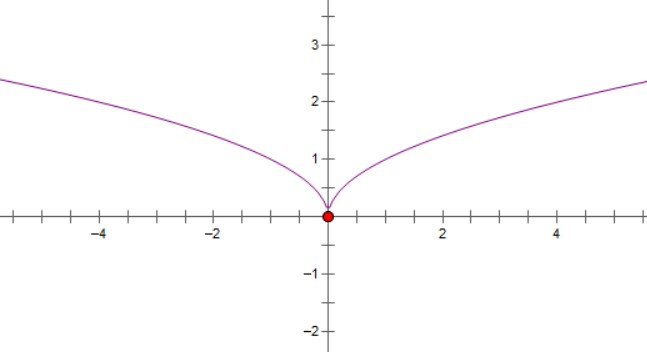
\includegraphics[width=.3\textwidth]{App2_3}
        \caption{原点不可导但是在原点取得极限值的一个例子.}\label{fig:原点不可导但是在原点取得极限值的一个例子.}
      \end{figure}

      \item 函数在某点处二阶可导且在该点处一阶导数为0、二阶导数不为0,是其在该点处取得极值的第二充分不必要条件. 该条件还可推广为在某点处偶数阶可导且除最高阶导数值外其他阶导数均为0.
    \end{enumerate}

  \subsection{二阶可导与凹凸性}
    \hspace*{2em}连续函数在某点处存在二阶导数,且该点处一阶导等于0、二阶导不等于0,不能推知函数在该点邻域内的凹凸性.

    如这样一题:设函数$f(x)$在$x = x_0$处存在二阶导数,且$f'(x_0)=0$, $f''(x_0)<0$,则必定存在$\delta > 0$使得(\qquad)
    \options{曲线$y=f(x)$在区间$(x_0 - \delta, x_0 + \delta)$上是凸的}
    {曲线$y=f(x)$在区间$(x_0 - \delta, x_0 + \delta)$上是凹的}
    {函数$f(x)$在区间$(x_0-\delta,x_0]$上严格单增,在区间$[x_0, x_0+\delta)$上严格单减}
    {函数$f(x)$在区间$(x_0-\delta,x_0]$上严格单减,在区间$[x_0, x_0+\delta)$上严格单增}
    答案:C. 对错解AB构造反例:$f\left( x \right) = \displaystyle\int_0^x{\left( t^2\sin \frac{1}{t}+\frac{t}{2} \right) \rd t}$.

  \subsection{后记}
    \hspace*{2em}以上举出的函数,有能力的话最好自己尝试作出图像或草图,以加深理解.
    最后留一道习题:讨论函数
    $f\left( x \right) =\begin{cases}
      ax^{\lambda}+bx^{\alpha}\sin \left( x^{\beta} \right), & x\ne 0 \\
      0, & x=0 \\
    \end{cases}\left( a,b,\alpha ,\beta ,\lambda \in \mathbb{R} \right)$
    在原点处存在几阶导数,各阶导函数在原点处是否连续.

\section{一元函数积分学部分}
~ \subsection{定积分与不定积分,可积与原函数,以及变限积分}
    \begin{enumerate}[label=(\arabic*)]
      \item 定积分存在$\Leftrightarrow$可积,不定积分存在$\Leftrightarrow$原函数存在.
      \item 不定积分和定积分是两个概念,不定积分存在不一定可积,可积也不一定有原函数.
      \item 变限积分借助微积分基本定理和Newton-Leibniz公式担当了沟通定积分和不定积分的桥梁,但要注意对被积函数的可积性/连续性、变限积分的连续性/可导性的区分.
    \end{enumerate}

  \subsection{可积(定积分存在)的三类条件}
    \begin{enumerate}[label=(\arabic*)]
      \item 必要不充分条件:有限区间上有界

      若不满足有限区间,立即成为无穷限的反常积分;若不满足有界,立即成为无界的反常积分. 对不满足充分性举例:狄利克雷函数在闭区间$[0,1]$上有界,但不可积.
      \item 充分不必要条件:
      \begin{enumerate}[label=(\roman*)]
        \item 闭区间上连续.

        注意和上文必要不充分条件里的“有限区间”区分开,前者可以是开区间(采用补充定义法立即变为闭区间),而这里必须是闭区间(开区间上的连续函数可能无界).
        \item 闭区间上有界,且只有有限个间断点.

        注意:第一,这里的间断点不能是无穷间断点;第二,教材上一般写为“且只有有限个第一类间断点”,并未讨论振荡间断点的情况. 实际上闭区间内含有有限个振荡间断点的有界函数也是可积的(但不一定有原函数),如
        $f\left( x \right) =\begin{cases}
          2x\sin \dfrac{1}{x}-\cos \dfrac{1}{x},&   x\ne 0\\
          0, &    x=0\\
        \end{cases}$
        在$[0,1]$上的定积分为$\sin 1$.
        对不满足必要性举例:函数$\sgn\left(\sin\dfrac{x}{\pi}\right)$在$[0,1]$上有无穷个间断点(一个振荡间断点$x = 0$以及可列无穷个跳跃间断点$x_k = \frac{1}{k}, k \in \mathbb{N}^\ast$),但可积. 具体为何可积将在充要条件里介绍.
        \item 闭区间上单调.
      \end{enumerate}
      \item 充要条件(注意,这部分超纲!)
      若定义在闭区间$[a,b]$上且有界的函数$f(x)$的全体间断点构成的集合是零测度集,则$f(x)$在$[a,b]$上(勒贝格)可积,逆命题也成立.

        注:把可以用总长度任意小的有限个区间覆盖的点集称为“零测度集”,简称零集. 上文中跳跃间断点$x_k = \frac{1}{k}, k \in \mathbb{N}^\ast$构成的集合是可数无穷集,故而为零测集.

      上述充要条件也表述为:区间上的有界函数可积的充要条件是几乎处处连续.
    \end{enumerate}

  \subsection{原函数(不定积分)存在的条件}
    \begin{enumerate}[label=(\arabic*)]
      \item 必要不充分条件:$f(x)$有原函数,则必定不含有第一类间断点或无穷间断点.
      \item 充分不必要条件:$f(x)$连续,则必定有原函数.
      \item 既非充分也非必要,需分类讨论:$f(x)$含有振荡间断点,则原函数不一定不存在.

      举例:$f\left( x \right) =\begin{cases}
        2x\sin \dfrac{1}{x}-\cos \dfrac{1}{x},&   x\ne 0\\
        0, &    x=0\\
      \end{cases}$
      有原函数
      $F\left( x \right) =\begin{cases}
        x^2\sin \dfrac{1}{x},&   x\ne 0\\
        0, &    x=0\\
      \end{cases}$.
    \end{enumerate}

\section{参考文献}
\begin{enumerate}[label={[\arabic*]}]
  \item 张宇等.~2019张宇高等数学18讲[M].北京:高等教育出版社,2017.12:120.
  \item 同济大学数学系.高等数学.第7版[M].北京:高等教育出版社,2017,9:59.
  \item 胡志兴等.高等数学.第2版[M].北京:高等教育出版社,2015.6:161.
  \item 谢惠民等.吉米多维奇数学分析习题集学习指引(第二册)[M].北京:高等教育出版社,2012,12:121-122.
  \item 谢惠民.数学分析习题课讲义上册[M].北京:高等教育出版社,2003:132
\end{enumerate}